\subsection{Учет защиты геостационарных систем}
\label{subsec:geoprotection}

Для учета защиты геостационарных систем \cite{ituRR2024,ituS1503_4} при
расчете покрытия земной поверхности спутниками Walker-построения будем
использовать геозащитную маску. Она применяется к каждой паре <<точка
поверхности -- КА>> и не зависит от способа разбиения поверхности Земли.
Рассмотрим произвольную точку $Q$ и зафиксируем момент времени. Все векторы
ниже задаются в системе координат ECEF. КА считается допустимым для точки $Q$,
если он удовлетворяет обычным условиям видимости из этой точки, а направление
на него достаточно удалено от всех видимых направлений на пояс ГСО.

Пусть $\mathbf r_Q=(x_Q,y_Q,z_Q)^{\mathsf T}$ -- радиус-вектор точки $Q$.
Пояс ГСО представим окружностью радиуса $R_{\mathrm{GEO}}$ в экваториальной
плоскости, параметризованной углом $\ell$:
\begin{equation}
    \mathbf g(\ell)=R_{\mathrm{GEO}}
    \begin{pmatrix}
        \cos \ell \\
        \sin \ell \\
        0
    \end{pmatrix},
    \qquad 0\leq \ell < 2\pi.
\end{equation}
Для эллипсоида WGS84 с экваториальной и полярной полуосями $a_{\oplus}$ и $b_{\oplus}$ направление внешней нормали в точке $Q$ задается вектором
\begin{equation}
    \mathbf n_Q=
    \begin{pmatrix}
        x_Q/a_{\oplus}^{2} \\
        y_Q/a_{\oplus}^{2} \\
        z_Q/b_{\oplus}^{2}
    \end{pmatrix}.
\end{equation}
Точка пояса ГСО видна из $Q$, если она находится над плоскостью локального горизонта или на ней. Поэтому множество соответствующих долгот определим как
\begin{equation}
    \mathcal{L}_{\mathrm{vis}}(Q)=
    \left\{
        \ell\in[0,2\pi):
        \bigl(\mathbf g(\ell)-\mathbf r_Q\bigr)\cdot\mathbf n_Q\geq 0
    \right\}.
    \label{eq:visible_geo_arc}
\end{equation}
Таким образом, $\mathcal{L}_{\mathrm{vis}}(Q)$ содержит видимую дугу и ее границы на локальном горизонте, а если пояс ГСО полностью скрыт Землей, это множество пусто (характерно для высоких широт).

Пронумеруем КА Walker-построения сквозным индексом $k=1,\ldots,PS$, обозначим $k$-й КА через $S_k$, а его радиус-вектор через $\mathbf r_k$. Единичные направления из точки $Q$ на КА и на произвольную точку пояса ГСО равны
\begin{equation}
    \mathbf d_k(Q)=
    \frac{\mathbf r_k-\mathbf r_Q}
         {\lVert\mathbf r_k-\mathbf r_Q\rVert_2},
    \qquad
    \mathbf d_{\mathrm{GEO}}(Q,\ell)=
    \frac{\mathbf g(\ell)-\mathbf r_Q}
         {\lVert\mathbf g(\ell)-\mathbf r_Q\rVert_2}.
\end{equation}
Каждому $\ell\in\mathcal{L}_{\mathrm{vis}}(Q)$ соответствует точка $G(\ell)$ видимой дуги ГСО с радиус-вектором $\mathbf g(\ell)$. Поэтому $\mathbf d_{\mathrm{GEO}}(Q,\ell)$ является единичным вектором вдоль луча из $Q$ в точку $G(\ell)$. При изменении $\ell$ этот луч последовательно направляется во все точки видимой дуги. Аналогично $\mathbf d_k(Q)$ задает направление из $Q$ на КА $S_k$. Эта геометрия показана на рис.~\ref{fig:geoprotection_geometry}.

\begin{figure}[ht]
    \centering
    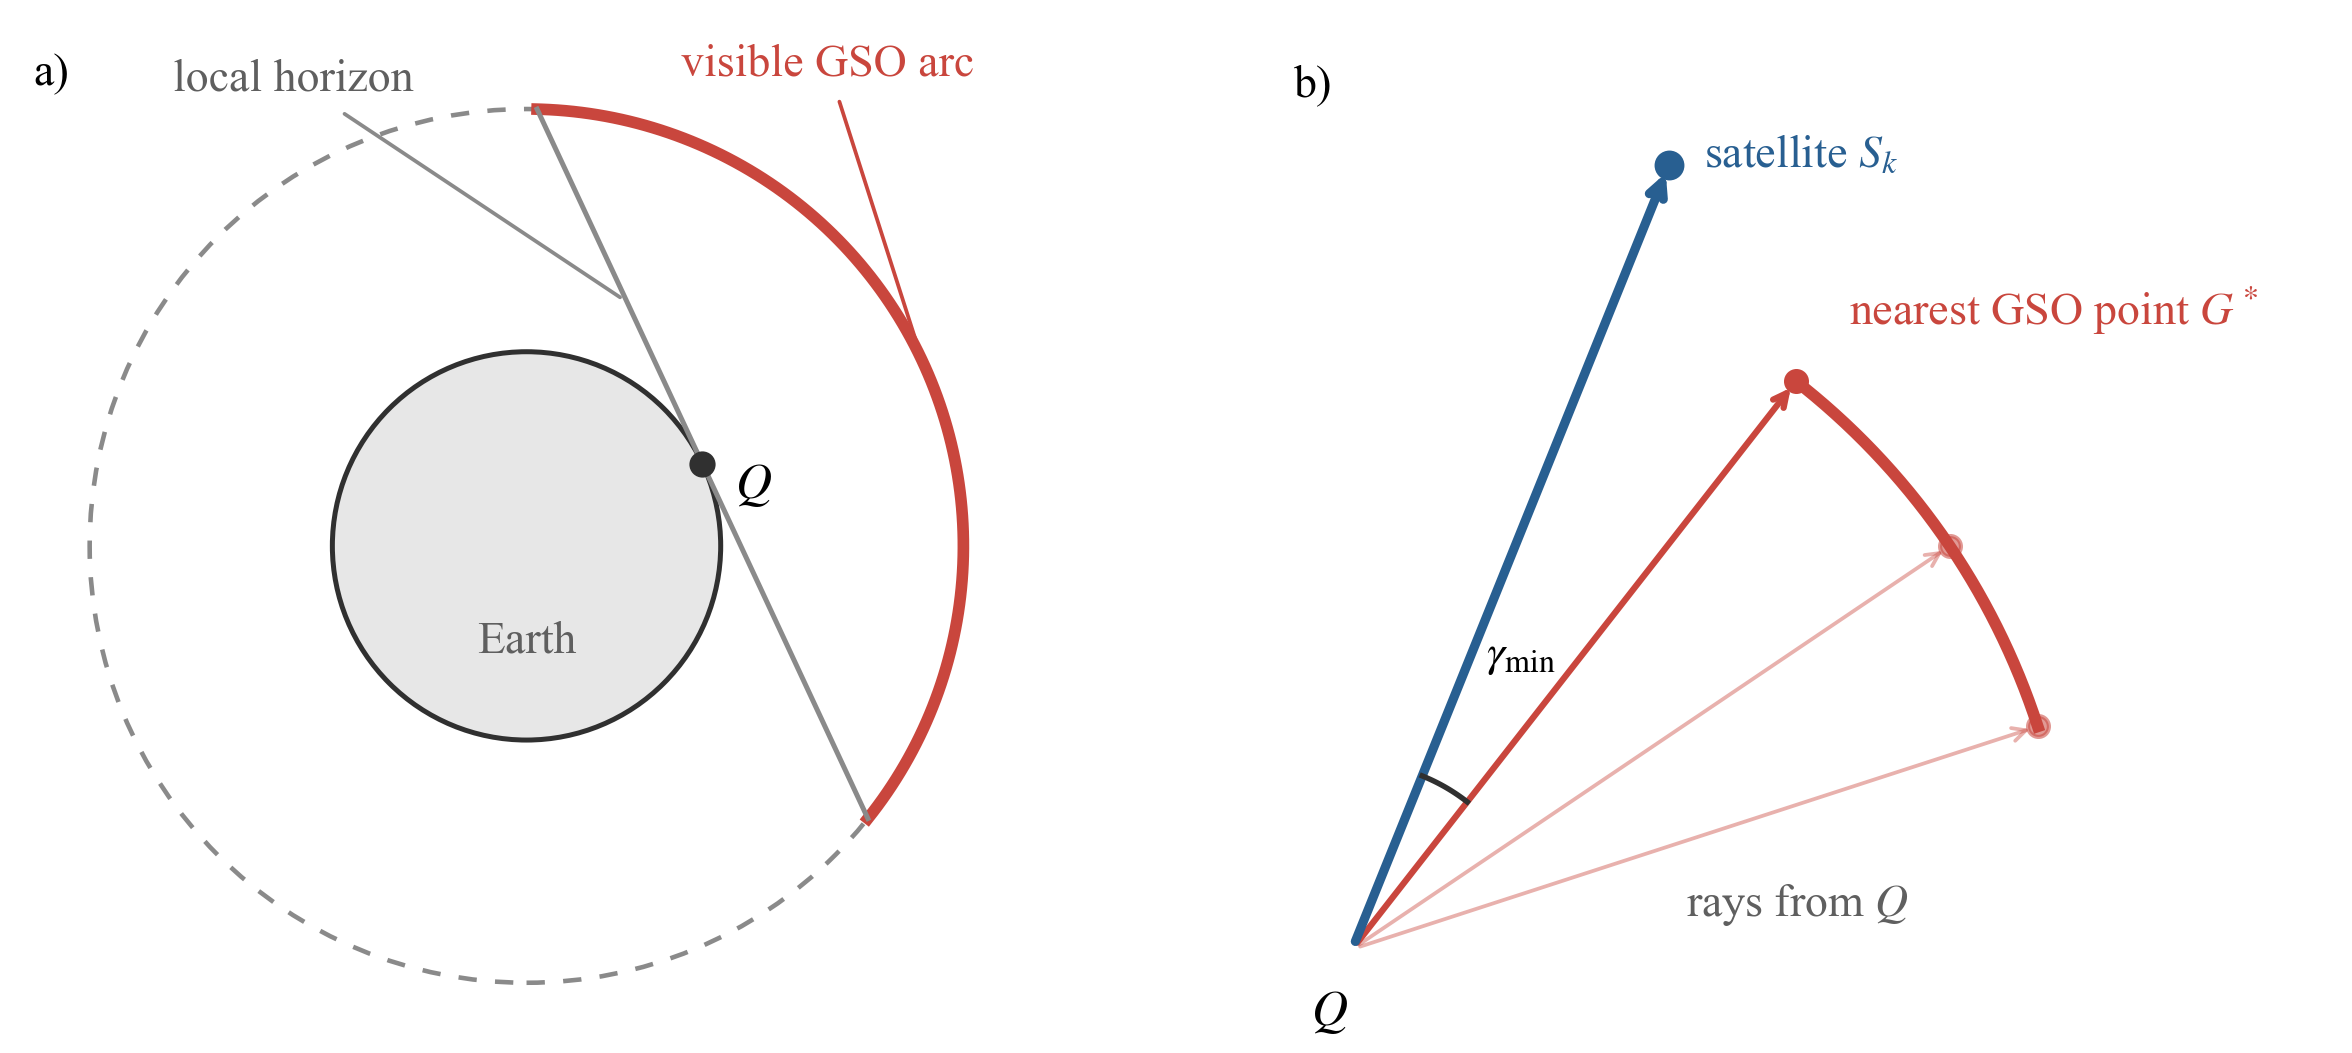
\includegraphics[width=\textwidth]{pictures/geoprotection_geometry.png}
    \caption{Схема геозащитной маски для произвольной точки $Q$ (не в масштабе):
    а) локальный горизонт выделяет видимую дугу ГСО; б) каждый красный луч
    соединяет $Q$ с одной из точек $G(\ell)$ этой дуги. Точка $G^*$ выбирается
    так, чтобы угол между лучами на $G^*$ и на КА $S_k$ был минимальным.}
    \label{fig:geoprotection_geometry}
\end{figure}

Минимальный угловой разнос между направлением на КА и видимой дугой ГСО можно определить как
\begin{equation}
    \gamma_{\min}(Q,k)=
    \min_{\ell\in\mathcal{L}_{\mathrm{vis}}(Q)}
    \arccos\left(
        \mathbf d_k(Q)\cdot\mathbf d_{\mathrm{GEO}}(Q,\ell)
    \right).
    \label{eq:minimum_geo_separation}
\end{equation}
\textcolor{red}{Практическая процедура вычисления минимума в \eqref{eq:minimum_geo_separation} описана в приложении \ref{app:geoprotection_angle_search}}.

Если видимая дуга существует, геозащитная маска пропускает пару $(Q,k)$ при выполнении условия
\begin{equation}
    \gamma_{\min}(Q,k)\geq\gamma_{\mathrm{GEO}},
    \label{eq:geoprotection_condition}
\end{equation}
где $\gamma_{\mathrm{GEO}}$ -- заданный угол геозащиты. Если из точки $Q$ пояс ГСО полностью скрыт Землей, это условие считается выполненным для любого видимого КА.

Таким образом, точка $Q$ считается покрытой, если в рассматриваемый момент существует хотя бы один КА, который одновременно удовлетворяет исходным условиям покрытия и условию \eqref{eq:geoprotection_condition}. Геозащитная маска не меняет геометрию зоны обзора отдельного КА, а исключает из расчета недопустимые пары <<точка поверхности -- КА>>.
